\documentclass[border=3pt,tikz]{standalone}
\usetikzlibrary{arrows,arrows.meta}
\usetikzlibrary{calc}
\usetikzlibrary{decorations.markings}
\usetikzlibrary{angles,quotes} % for pic (angle labels)
%\usepackage{tkz-euclide} % for \tkzMarkRightAngle
%\usetkzobj{all}
\tikzset{>=latex} % for LaTeX arrow head

\colorlet{myblue}{blue!80!black}
\colorlet{mydarkblue}{blue!35!black}
\colorlet{myred}{black!50!red}
\colorlet{glasscol}{blue!10}
\colorlet{Ecol}{orange!90!black}
\tikzstyle{myarr}=[-{Latex[length=3,width=2]}]
\tikzstyle{Evec}=[Ecol,{Latex[length=2.8,width=2.5]}-{Latex[length=2.8,width=2.5]},line width=0.6]
\tikzstyle{glass}=[top color=glasscol!88!black,bottom color=glasscol,shading angle=0]
%\tikzstyle{glass}=[top color=glasscol!88!black,bottom color=glasscol,middle color=glasscol!98!black,shading angle=0]
\tikzset{
  light beam/.style={thick,myblue,decoration={markings,
                     mark=at position #1 with {\arrow{latex}}},
                     postaction={decorate}},
  light beam/.default=0.5}

\newcommand\rightAngle[4]{
  \pgfmathanglebetweenpoints{\pgfpointanchor{#2}{center}}{\pgfpointanchor{#3}{center}}
  \coordinate (tmpRA) at ($(#2)+(\pgfmathresult+45:#4)$);
  \draw[white,line width=0.6] ($(#2)!(tmpRA)!(#1)$) -- (tmpRA) -- ($(#2)!(tmpRA)!(#3)$);
  \draw[blue!40!black] ($(#2)!(tmpRA)!(#1)$) -- (tmpRA) -- ($(#2)!(tmpRA)!(#3)$);
}


\begin{document}

% INTERNAL REFLECTION: almost
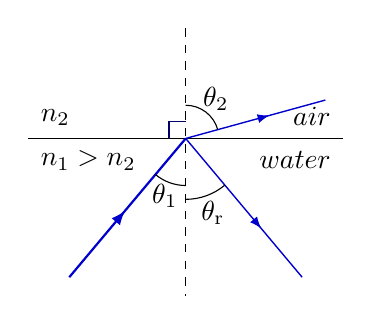
\begin{tikzpicture}
  \def\L{4.0}
  \def\l{2.3}
  \def\t{0.5}
  \def\h{2.0}
  \def\f{0.5}
  \def\na{1.0} % air
  \def\ng{1.5} % glass
  \def\angg{40} % asin(1/1.5)*180/pi
  \def\anga{asin(\ng/\na*sin(\angg))}
  \coordinate (O) at (0,0);
  \coordinate (I) at (-90-\angg:\l);
  \coordinate (M) at (-90+\angg:\l);
  \coordinate (F) at ({90-\anga}:0.8*\l);
  \coordinate (L) at (-\f*\L,0);
  \coordinate (R) at ({(1-\f)*\L},0);
  \coordinate (T) at (0,0.7*\h);
  \coordinate (B) at (0,-\h);
  
  % MEDIUM
  % \fill[glass] (L) rectangle++ (\L,-\t); % glass gradient
  % \fill[glasscol] (-\f*\L,-0.99*\t) rectangle ({1-\f)*\L},-\h);
  %\fill[glass] (L) rectangle (\L/2,-\h);
  \draw[] (L) -- (R);
  \node[above right=1] at (L) {$n_2$};
  \node[below right=1] at (L) {$n_1>n_2$};
  \node[above left=1] at (R) {$air$};
  \node[below left=1] at (R) {$water$};

  % LINES
  \draw[dashed] (T) -- (B);
  \draw[light beam={0.48}] (I) -- (O);
  \draw[light beam={0.65},line width=0.5] (O) -- (M);
  \draw[light beam={0.60},line width=0.5] (O) -- (F);
  
  % ANGLES
  \draw pic["$\theta_1$",draw=black,angle radius=17,angle eccentricity=1.3] {angle = I--O--B}; %\contour{white}{
  \draw pic["$\theta_\mathrm{r}$",draw=black,angle radius=22,angle eccentricity=1.3] {angle = B--O--M};
  \draw pic["$\theta_2$",draw=black,angle radius=12,angle eccentricity=1.5] {angle = F--O--T};
  \rightAngle{L}{O}{T}{0.3}
  
\end{tikzpicture}


\end{document}